\documentclass{article}
\usepackage[utf8]{inputenc}
\usepackage{amsmath,amssymb}
\usepackage{parskip}
\usepackage{graphicx}
\usepackage{eurosym}


% Margins
\usepackage[top=2.5cm, left=3cm, right=3cm, bottom=4.0cm]{geometry}
% Colour table cells
\usepackage[table]{xcolor}

% Get larger line spacing in table
\newcommand{\tablespace}{\\[1.25mm]}
\newcommand\Tstrut{\rule{0pt}{2.6ex}}         % = `top' strut
\newcommand\tstrut{\rule{0pt}{2.0ex}}         % = `top' strut
\newcommand\Bstrut{\rule[-0.9ex]{0pt}{0pt}}   % = `bottom' strut

%%%%%%%%%%%%%%%%%
%     Title     %
%%%%%%%%%%%%%%%%%
\title{Theory of automata and Formal languages}
\author{Fernando Javier López Cerezo \\ Practice 1}
\date{\today}

\begin{document}
\maketitle

%%%%%%%%%%%%%%%%%
%   Problem 1   %
%%%%%%%%%%%%%%%%%
\section*{Exercise 1}
Let $R=\{(1,1),(1,2),(2,3),(3,4)\}$ be a binary relation. Exercise 1 asks us to find $R^3$. \\$R^2 = \{(a,b) : \exists x \in A, (a,x) \in R \land (x,b) \in R\} = \{(1,1),(1,2),(1,3),(2,4)\}$ \\ $R^3 = \{(a,b) : \exists x \in A, (a,x) \in R^2 \land (x,b) \in R\} = \{(1,1),(1,2),(1,3),(1,4)\}$ \\\\ Checking the answer with Octave: \\\\ 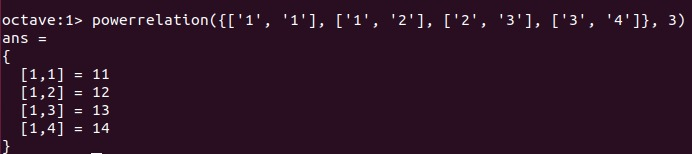
\includegraphics[width=\linewidth]{octave.png}


\end{document}